\documentclass[tikz,border=2pt]{standalone}
\usepackage{amsmath,amssymb}
\usepackage{tikz}
\usetikzlibrary{arrows.meta}

\begin{document}
% Dividing complex numbers divides the moduli and subtracts the arguments.
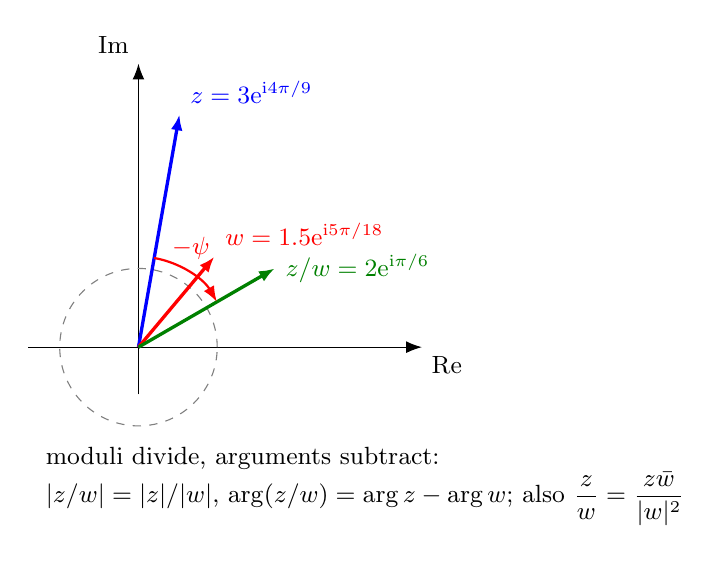
\begin{tikzpicture}[every node/.style={font=\small}, >={Latex[length=2mm]}]
	\draw[->] (-1.4,0) -- (3.6,0) node[below right] {$\mathrm{Re}$};
	\draw[->] (0,-0.6) -- (0,3.6) node[above left] {$\mathrm{Im}$};
	\draw[gray, dashed] (0,0) circle (1);
	\draw[->, blue, very thick] (0,0) -- (80:3) node[above right] {$z=3\mathrm{e}^{\mathrm{i}4\pi/9}$};
	\draw[->, red, very thick] (0,0) -- (50:1.5) node[above right] {$w=1.5\mathrm{e}^{\mathrm{i}5\pi/18}$};
	\draw[->, green!50!black, very thick] (0,0) -- (30:2) node[right] {$z/w=2\mathrm{e}^{\mathrm{i}\pi/6}$};
	\draw[red, thick, ->] (80:1.15) arc (80:30:1.15);
	\node[red, font=\small] at (62:1.42) {$-\psi$};
	\node[anchor=north west, align=left] at (-1.3,-1.15) {moduli divide, arguments subtract:\\ $|z/w|=|z|/|w|$, $\arg(z/w)=\arg z-\arg w$; also $\dfrac zw=\dfrac{z\bar w}{|w|^2}$};
\end{tikzpicture}
\end{document}
